\documentclass[11pt]{article}
\usepackage[utf8]{inputenc}
\usepackage[spanish,es-tabla]{babel}
\usepackage[margin=35mm]{geometry} %Márgenes mas pequeños
\usepackage{cite}
\usepackage{amsmath,amssymb,amsfonts}
\usepackage{algorithmic}
\usepackage{graphicx}
\usepackage{textcomp}
\usepackage{xcolor}
\usepackage{booktabs}
\usepackage{optidef}
\usepackage{pdfpages}
\usepackage{float}
\restylefloat{table}
\usepackage{tocloft}
\renewcommand{\cftsecleader}{\cftdotfill{\cftdotsep}} %ToC con puntos en todos
\usepackage{minted}
\graphicspath{{res/}}




\def\BibTeX{{\rm B\kern-.05em{\sc i\kern-.025em b}\kern-.08em
    T\kern-.1667em\lower.7ex\hbox{E}\kern-.125emX}}
%Lo de arriba son como imports, no le heches cuenta ;)

\title{
        \textbf{TweetKell}\\
        \medskip
        \large{Análisis de los datos privados de una cuenta de Twitter con Haskell}\\
        \bigskip
        Universidad de Sevilla\\ Ingeniería Informática Tecnologías Informáticas\\
        Programación Declarativa - Tercer curso}
        
\author{
Juan Arteaga Carmona\\
Herrera, Sevilla, España \\
\texttt{JuanArteaga@andalu30.me}\\
}



\begin{document}

%Portada con titulo e integrantes
\maketitle
\newpage

%Índice de la memoria
\tableofcontents
% \listoftables
\listoffigures
\newpage

%Documento----
\section{Introducción}
A continuación se presenta la documentación realizada para la entrega final de la convocatoria de Septiembre del trabajo de curso de la asignatura Programación Declarativa del grado de Ingeniería Informática - Tecnologías Informáticas de la Universidad de Sevilla.

\section{Expectativas}
Al comienzo del trabajo se pretendía obtener una versión final que cumpliese con los requisitos expuestos por nuestro profesor, los cuales se pueden observar en el apartado \ref{apt:criterios}.

\section{Criterios de evaluación}\label{apt:criterios}
A continuación se muestran los criterios de evaluación a los que se someterá este trabajo, de acuerdo con la información que se encontraba en el aula virtual de la asignatura a día 2 de septiembre de 2019.

\begin{itemize}
    \item La fecha de entrega del trabajo es el día 8 de septiembre hasta media noche. La defensa del trabajo tendrá lugar la semana siguiente, del 9 al 13 (se anunciará por este canal las fechas).
    \item El trabajo debe ser un programa de temática "libre" (dentro de los ofertados en la convocatoria de febrero, o los que se haya hablado con los profesores previamente), totalmente funcional. Para la superación del trabajo, éste debe contener como mínimo:
    
    \begin{itemize}
        \item Dos aplicaciones de cada concepto básico de programación funcional visto en cada tema del primer bloque de la asignatura (temas 2,4,5,6,7,8). Es decir: al menos usar 2 funciones básicas de haskell, definir 2 funciones recursivas, 2 funciones por patrones, 2 usos de guardas, 2 usos de listas por comprensión, 2 usos de orden superior, 2 usos de tipados, etc.
    \item Creación de un módulo
    \item Creación de un tipo de datos nuevo y uso de éste.
    \item Uso de al menos dos de los conceptos avanzados y librerías vistos en los temas 3, 9, 11, 12, 13, 14 o 15 (deben ser de temas distintos).
    \end{itemize}
    
    
    \item La entrega debe contener, en un archivo comprimido (zip, máximo 50 mb):
    \begin{itemize}
        \item El código fuente Haskell (incluyendo un pequeño readme explicando el uso del programa).
        \item Un documento (formato libre) explicando la estructura del código y cómo se ha aplicado cada uno de los conceptos.
    \end{itemize}


\end{itemize}

\section{Elección del tipo de trabajo}
Se decidió que el trabajo fuese uno completamente diferente al que se propuso en la primera convocatoria \cite{trabajoPrimeraConv} ya que, tal y como se explicó en las conclusiones de este, elaborar un juego con Haskell y CodeWord no parecía ser una tarea sencilla ni interesante. 

Así pues, este trabajo se centrara en la temática de Data Science y análisis de datos, con especial énfasis en la recolección de los datos a través de la librería Aeson \cite{Aeson} y en la interactividad del programa como se verá en el apartado \ref{aplicacionConceptos}.


\section{Haskell}
Para este proyecto utilizaremos en lenguaje de programación Haskell\cite{haskellweb}.
Haskell es un lenguaje de programación puramente funcional creado por Paul Hodax en 1990 \cite{origenhaskell}.


\section{Datos de Twitter}
Al utilizar esta aplicación podremos extraer y consultar los datos de una cuenta de Twitter, para esto es necesario que dispongamos de los datos en un formato que nuestro PC pueda entender.

Para conseguir los datos deberemos de hacer a Twitter una petición para que nos permita descargarlos. Esta petición se hace a traves de los ajustes de privacidad en nuestro perfil y, dependiendo del tamaño de nuestra cuenta, en unos minutos se nos permitirá acceder a ellos. \cite{twitterData}

Una vez descargados, tendremos que descomprimirlos y ya podremos utilizar la aplicación.

\section{Implementación}
\subsection{Estructura del código}
El código se encuentra estructurado en varios módulos que, además de ser un requisito para la entrega del trabajo, permiten una mayor comodidad y simplicidad a la hora de desarrollar la aplicación.
A continuación se describen los módulos:
 \begin{itemize}
     \item \mint{haskell} TweeKell.hs
     Archivo principal del programa, contiene una función main que llama al menu principal del módulo MenuInteractivo.
     
     \item \mint{haskell} MenuInteractivo.hs
     Módulo encargado de generar los menús interactivos del programa además de recibir las instrucciones del usuario y llamar a la lógica correcta.
     
     \item \mint{haskell} TiposDatos.hs
     Módulo encargado de definir los tipos de datos que se utilizan para decodificar los archivos JSON y mostrar la información.
     
     \item \mint{haskell} TiposDatos2.hs
     Igual que TiposDatos, con la única diferencia de que este contiene las definiciones de los tipos de datos que producen alguna colisión en caso de que se encontrasen en TiposDatos.
     
     \item \mint{haskell} ParsersArchivos.hs
     Módulo encargado de parsear los archivos JSON de Twitter y de crear los objetos de los tipos que se definen en TiposDatos y TiposDatos2.
     
     \item \mint{haskell} AnalisisSimples.hs
     Módulo encargado de recibir el parseado realizado por ParsersArchivos y analizar y mostrar la información que el usuario ha solicitado para todos los tipos de análisis excepto para los que dependen de Tweets.
     
     \item \mint{haskell} AnalisisTweets.hs
     Igual que AnalisisSimples pero centrado en los que dependen del tipo Tweet.
 \end{itemize}


\subsection{Aplicación de los conceptos y ajuste a los criterios de evaluación}\label{aplicacionConceptos}

\begin{itemize}
    \item \textbf{Aplicaciones de conceptos básicos de programación funcional.}
    \begin{itemize}
        \item 2 funciones básicas de Haskell
        
        El uso de funciones básicas de Haskell se puede observar por todo el trabajo, por ejemplo, se puede observar en dos de las funciones mas simples y cortas:
        \medskip
        \begin{minted}[frame=lines,framesep=2mm,fontsize=\footnotesize,linenos]{haskell}
modPhoneFile :: String -> String
modPhoneFile string ="{" ++ (drop 50 $ reverse $ drop 4 $ reverse string)

modAccFile :: String -> String
modAccFile string = drop 45 $ reverse $ drop 3 $ reverse string
        \end{minted}
        \medskip
        
        \item 2 funciones recursivas:
        
        A continuación podemos ver dos funciones recursivas de este trabajo, una de ellas se encarga de imprimir los textos de una lista de Tweets y otra se encarga de contar el número de apariciones de los distintos idiomas de los tweets.
        
        \begin{minted}[frame=lines,framesep=2mm,fontsize=\footnotesize,linenos]{haskell}
        imprimeTextosTweets :: [String] -> IO()
        imprimeTextosTweets [] = putStrLn "" --Base
        imprimeTextosTweets (x:ls) = do  --Recursiva
          putStr "\n->"
          print x
          imprimeTextosTweets ls
          
        cuentaIdiomas :: Foldable t => [t a] -> [Int] -> [Int]
        cuentaIdiomas [] ac = ac
        cuentaIdiomas (x:xs) ac = do
          let newac = ac ++ [(length x)]
          cuentaIdiomas xs newac
            \end{minted}
        \medskip
        \item 2 funciones por patrones
        
        Las dos funciones recursivas anteriores están, claramente, definidas por patrones. Sin embargo no son las únicas. Un ejemplo de otra función sería el siguiente:
        \begin{minted}[frame=lines,framesep=2mm,fontsize=\footnotesize,linenos]{haskell}
tipoAnalisis :: String -> [String]
tipoAnalisis "account.js" = ["1: Ver informacion", "2: Abrir en navegador"]
tipoAnalisis "profile.js" = ["1: Ver informacion","8: Ver icono de perfil"]
tipoAnalisis "verified.js" = ["1: Ver informacion"]
tipoAnalisis "phone-number.js" = ["1: Ver informacion"]
tipoAnalisis "tweet.js" = ["3: Ver tweets", "4: Ver Retweets", "5: Tweet mas retweeteado",
                           "6: Tweet con más MG","7: Idiomas mas utilizados"]
            \end{minted}

        \medskip
        \item 2 usos de guardas
        
        En cuanto a funciones con guardas, dos ejemplos podrían ser:
        
        \begin{minted}[frame=lines,framesep=2mm,fontsize=\footnotesize,linenos]{haskell}
verInformacion :: String -> String -> IO()
verInformacion ruta archivo
  | archivo == "account.js" = verInformacionAccount (ruta ++"/"++ archivo)
  | archivo == "profile.js" = verInformacionProfile (ruta ++"/"++ archivo)
  | archivo == "verified.js" = verInformacionVerified (ruta ++"/"++ archivo)
  | archivo == "phone-number.js" = verInformacionPhone (ruta ++"/"++ archivo)
  
abrirNavegador :: String -> String -> IO()
abrirNavegador ruta archivo
  | archivo == "account.js" = abrirNavegadorAccount (ruta ++"/"++ archivo)
  | archivo == "profile.js" = abrirNavegadorAccount (ruta ++"/"++ archivo)
            \end{minted}
        
        \item 2 usos de tipados
        
        En cuanto al uso de tipados, debido a que Haskell es un lenguaje fuertemente tipado se deben de usar sin excepción. En las funciones de ejemplo anteriores se puede ver como, además, se escribe el tipo de la función para que el lenguaje nisiquiera tenga que inferirlo.
        
        
    \end{itemize}
    
    \item \textbf{Creación de al menos un módulo}
    
    Un ejemplo de la creación de un módulo en este trabajo sería el módulo TiposDatos, que se encarga de definir parte de los distintos tipos de datos que se usan en el trabajo.
    
    \item \textbf{Creación de un tipo de datos y uso de este}
    
    Utilizando el mismo archivo que en el apartado anterior, podemos ver varias definiciones de tipos de datos, por ejemplo uno de los mas interesantes sería el tipo de datos Tweet:
    
        \begin{minted}[frame=lines,framesep=2mm,fontsize=\footnotesize,linenos]{haskell}
            data Tweet = Tweet {
              favorite_count :: String,
              retweet_count :: String,
              created_at :: String,
              full_text :: String,
              lang :: String
            } deriving (Generic, Show)
            instance FromJSON Tweet
        \end{minted}
        
    En este tipo de datos recogemos 5 de entre todos los parámetros que nos encontramos en los archivos de Twitter.
    
    
    \item \textbf{Uso de dos conceptos avanzados}
    
    En cuanto a uso de conceptos avanzados, como este trabajo se centraba en Data Science y analisis de datos, uno de los mas importantes ha sido el procesamiento de archivos JSON con Aeson
    \begin{itemize}
        \item Procesamiento JSON con Aeson:
        
        Para decodificar archivos JSON se ha usado la libreria Aeson\cite{Aeson}, que nos ha permitido recojer los datos de los archivos sin problemas.
        Todo esto se ha realizado con las distintas funciones del archivo \textit{ParsersArchivos.hs}. A continuación podemos ver un ejemplo de parseado de los Tweets.
        
        \begin{minted}[frame=lines,framesep=2mm,fontsize=\footnotesize,linenos]{haskell}
            parseTweets :: String -> IO [Tweet]
            parseTweets path = do
              preparaTweets path
              file <- B.readFile (path++".mod")
              let tweets = decode file :: Maybe [Tweet]
              case tweets of
                Nothing -> exitSuccess
                Just tweets -> return tweets
        \end{minted}
        \medskip
        \item Programa interactivo:
        
        En cuanto al segundo concepto avanzado, la primera idea fue utilizar la documentación de la asignatura para intentar implementar una paralelización sencilla. Sin embargo, finalmente se decidió implementar un programa interactivo, ya que sería una solución mas sencilla y rápida, además de que el tamaño de los datos de una cuenta de Twitter, especialmente de la parte que analizamos nosotros, no es tan grande como para necesitar paralelismo o clustering.
        
        Esta interactividad se hace con las funciones del módulo \textit{MenuInteractivo.hs}, por ejemplo, aqui podemos ver el menú principal de la aplicación:
        
        \begin{minted}[frame=lines,framesep=2mm,fontsize=\footnotesize,linenos]{haskell}
            menuPrincipal :: IO()
            menuPrincipal = do
              clearScreen
              putStrLn "Hola, bienvenido al wizard de TweeKell"
              putStrLn "Menu principal:"
              putStrLn "Pulse enter para comenzar o escriba alguna opción"
            
              putStrLn "\ni: Información"
              putStrLn "q: Salir"
            
              option <- getLine
              case option of
                "i" -> menuInformacion
                "q" -> exitSuccess
                _ -> menu1
        \end{minted}
        
        Como se puede observar, se espera la interacción del usuario y se responde correctamente dependiendo de lo elegido.
        
        
        
    \end{itemize}
    
\end{itemize}

\section{Uso de la aplicación}
Para usar la aplicación se puede ejecutar el archivo compilado en cualquier sistema GNU/Linux o, si se prefiere, se puede utilizar el código fuente.
Una vez ejecutado deberiamos de ver el menu principal de la aplicación tal y como muestra la figura \ref{fig_menuprincipal}.

\begin{figure}[h]
    \centering
    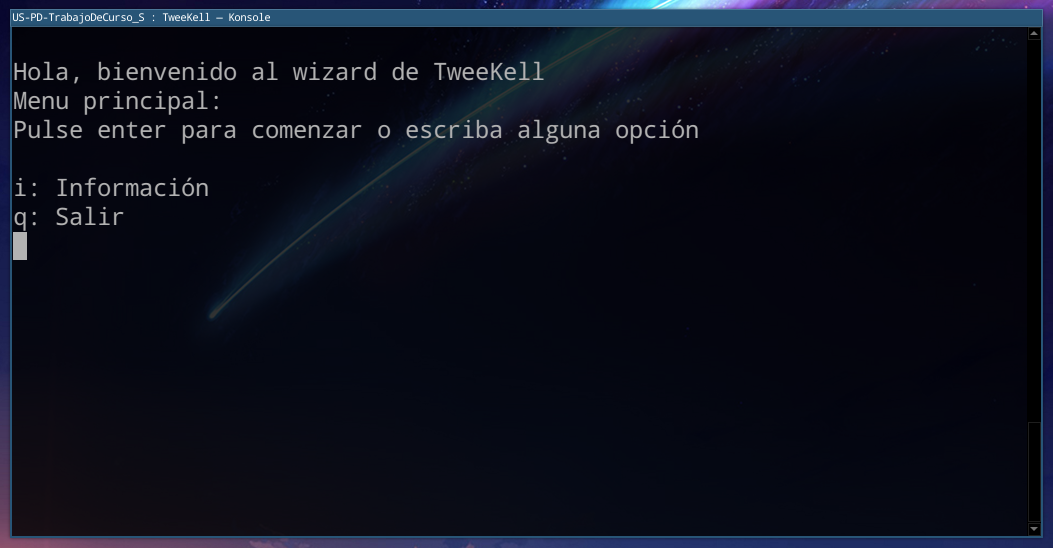
\includegraphics[width=0.75\textwidth]{menuPrincipal.png}
    \caption{Menú principal de la aplicación}
    \label{fig_menuprincipal}
\end{figure}
\medskip

A continuación, siguiendo los menus introduciremos la ruta al archivo que queremos analizar y comprobaremos que lo hemos introducido correctamente tal y como se ve en la figura \ref{fig_comprobacion}

\begin{figure}[h]
    \centering
	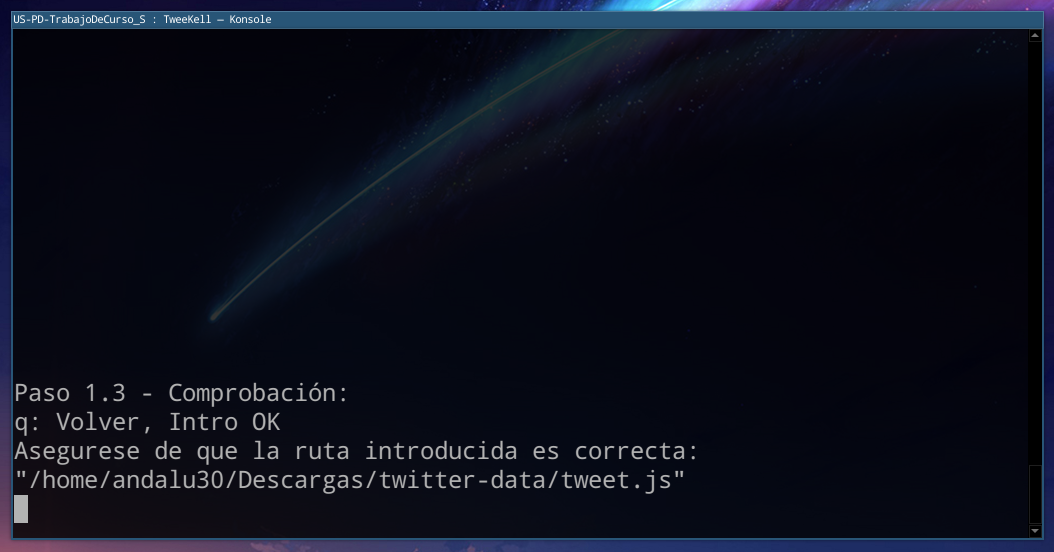
\includegraphics[width=0.75\textwidth]{comprobacion.png}
    \caption{Pantalla de confirmación de la ruta del archivo a analizar}
    \label{fig_comprobacion}
\end{figure}
\medskip

Tras esto, podremos seleccionar el tipo de análisis que queremos realizarle al archivo, un ejemplo que podemos ver en la figura \ref{fig_tipoAnalisis} serían los tipos de analisis sobre el archivo \textit{Tweet.js}

\begin{figure}[h]
    \centering
    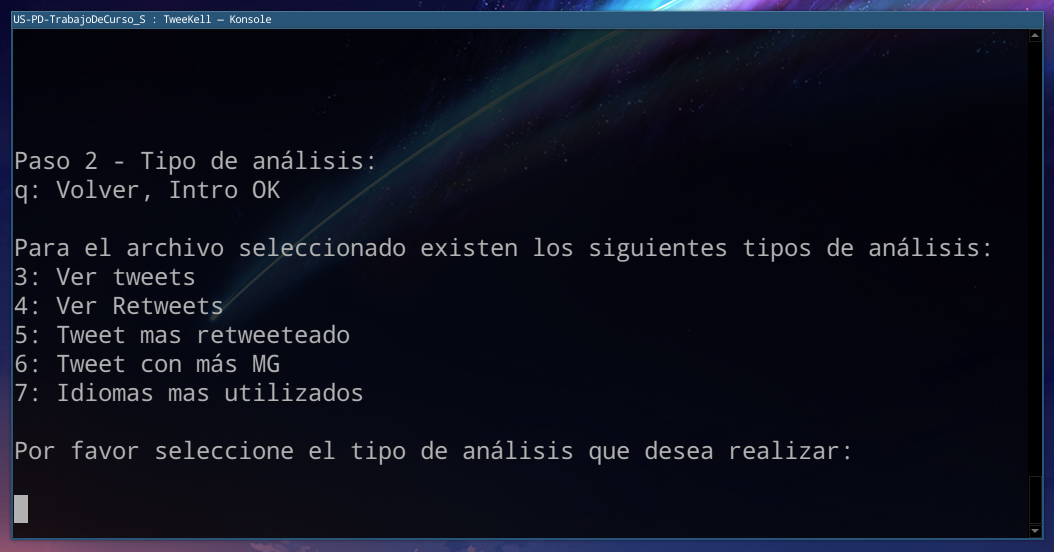
\includegraphics[width=0.75\textwidth]{tiposanalisis.png}
    \caption{Distintos tipos de análisis que se pueden realizar sobre el archivo \textit{Tweet.js}}
    \label{fig_tipoAnalisis}
\end{figure}
\medskip

Finalmente, tras seleccionar el tipo de análisis que queremos ver nos encontraremos con una pantalla que nos presentará los resultados. Un ejemplo seria la pantalla de la figura \ref{fig_resultados}

\begin{figure}[h]
    \centering
    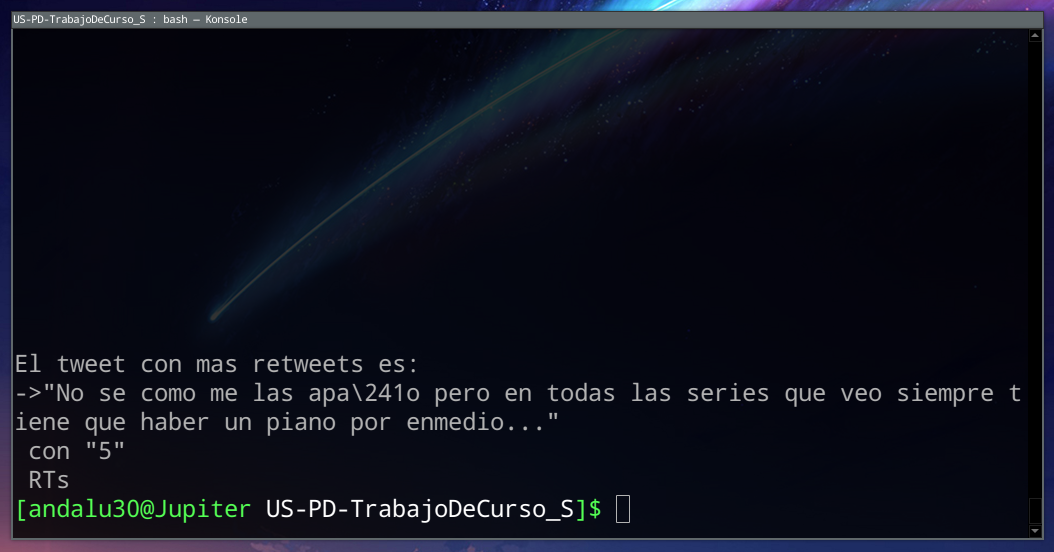
\includegraphics[width=0.75\textwidth]{analisisdone.png}
    \caption{Pantalla de resultados del análisis}
    \label{fig_resultados}
\end{figure}



\subsection{Utilizando el archivo compilado}
El archivo compilado \textit{TweeKell} se debe de poder ejecutar en cualquier sistema GNU/Linux sin problemas\footnote{Testeado en varios sistemas corriendo Fedora Workstation, Manjaro Linux, Ubuntu Server y Arch Linux} mediante la ejecución del comando \textit{./Tweekell}. Tras esto podremos ver el menu principal tal y como se ve en la figura \ref{fig_menuprincipal}

\subsection{Utilizando el código fuente}
Si se prefiere utilizar el código fuente para ejecutar la aplicación se podrá, por ejemplo, utilizar ghci. En este caso, ejecute \textit{ghci} en una terminal, cargue el archivo \textit{TweeKell.hs} con \textit{:l Tweekell.hs} y ejecute \textit{main}, debería de ver el menu principal.


\section{Posibles mejoras}
\subsection{Analizar más información}

Una de las posibles mejoras a este trabajo, sería la de analizar más información de la que se analiza actualmente. De entre los 45 archivos que Twitter nos ofrece, apenas analizamos 5 de ellos.
Los archivos más interesantes de analizar serian posiblemente \textit{like.js}, \textit{ad-engagement.js} y \textit{ad-impressions.js}.

\subsection{Paralelización y computación distribuida}
Otra posible mejora al trabajo sería la implementación de paralelismo en los análisis para que de esta forma podamos aprovechar la gran potencia de los PCs actuales. 

Otra forma de escalar nuestra aplicación para que soporte grandes cantidades de datos sería la de utilizar computación distribuida. Un ejemplo de esto sería Apache Spark\cite{spark}, que nos permitiría crear clusters para poder analizar una gran cantidad de información.


%Bibliografía
\begin{thebibliography}{99}

\bibitem{trabajoPrimeraConv} Juan Arteaga Carmona \textit{Recreando un juego interactivo con Haskell y CodeWorld-API} \href{https://github.com/Andalu30/US-PD-TrabajoDeCurso}{github.com/Andalu30/US-PD-TrabajoDeCurso - Repositorio privado en GitHub}

\bibitem{Aeson} Bryan O'Sullivan. \textit{Aeson: A fast Haskell JSON library} \href{https://github.com/bos/aeson}{github.com/bos/aeson - Repositorio en GitHub}

\bibitem{haskellweb} Paul Hudak, \textit{Haskell} \href{https://www.haskell.org/}{ Web del lenguaje}.

\bibitem{origenhaskell} Hudak, Paul; Hughes, John; Peyton Jones, Simon; Wadler, Philip (2007), \textit{A History of Haskell: Being Lazy with Class} ISBN 978-1-59593-766-7.

\bibitem{twitterData} Twitter \textit{Cómo acceder a tus datos de Twitter} \href{https://help.twitter.com/es/managing-your-account/accessing-your-twitter-data}{Enlace a la web de asistencia de Twitter}

\bibitem{spark} The Apache Software Foundation \textit{Apache Spark, Lightning-fast unified analytics engine} \href{https://spark.apache.org
}{Enlace a la web}




\end{thebibliography}


\end{document}
